\documentclass{article} % \documentclass{} is the first command in any LaTeX code.  It is used to define what kind of document you are creating such as an article or a book, and begins the document preamble

\usepackage{amsmath} % \usepackage is a command that allows you to add functionality to your LaTeX code
\usepackage{graphicx}
\graphicspath{ {./images/} }
\title{Discrete Time Signals and Systems} % Sets article title
\author{Hunter Mills} % Sets authors name
\date{\today} % Sets date for date compiled

% The preamble ends with the command \begin{document}
\begin{document} % All begin commands must be paired with an end command somewhere
    \maketitle % creates title using information in preamble (title, author, date)
    
    \section{Discrete Time Signals} % creates a section
    
    \subsection{Some Elementary DT Signals}
    The following signals appear often and play an important rule in DT signals and systems.
    
    \textbf{1.} The \textit{unit sample sequence} (delta function) if denoted as $\delta$(n) and is defined as:
    \begin{equation}
 	 \delta (n) =
    	\begin{cases}
      	1, & \text{for n = 0}\\
      	0, & \text{for n } \neq \text{0}
    	\end{cases}       
	\end{equation}
    
    \begin{figure}[h]
    \centering
	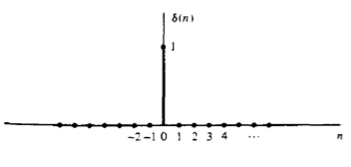
\includegraphics[width=10cm]{delta}
	\caption{Delta Signal}
	\end{figure}
	This signal is zero everywhere except at $n = 0$ where its value is 1.
	
	\textbf{2.} The \textit{unit step} signal is denoted as $u(n)$ and is defined as:
	\begin{equation}
 	 u(n) =
    	\begin{cases}
      	1, & \text{for n } \ge { 0}\\
      	0, & \text{for n } < { 0}
    	\end{cases}       
	\end{equation}
    
    \begin{figure}[h]
    \centering
	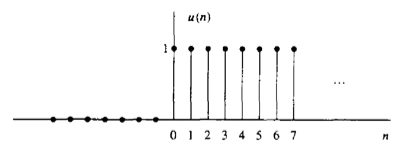
\includegraphics[width=10cm]{step}
	\caption{Unit Step Signal}
	\end{figure}
	
	\textbf{3.} The \textit{unit ramp} signal is denoted as $u_r(n)$ and is defined as:
	\begin{equation}
 	 u_r(n) =
    	\begin{cases}
      	n, & \text{for n } \ge { 0}\\
      	0, & \text{for n} <{ 0}
    	\end{cases}       
	\end{equation}
    
    \begin{figure}[h]
    \centering
	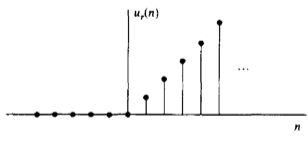
\includegraphics[width=10cm]{ramp}
	\caption{Unit Ramp Signal}
	\end{figure}
	
	\textbf{4.} The exponential signal is a sequence of the form
	\begin{equation}
 	 x(n) = a^n \;\;\;\; \text{for all } n
	\end{equation}
	If (a) is a real number then x(n) will be a real signal. (a) can also be a complex number defied as:
	\begin{equation}
 	a = re^{j\theta}
	\end{equation}
	where r and $\theta$ are now the parameters, which gives:
	\begin{equation}
 	 x(n) = r^ne^{j\theta n}
	\end{equation}
	\begin{equation}
 	 x(n) = r^n(\cos \theta n + j\sin \theta n)
	\end{equation}
	This equation can then be broken down into the real and imaginary parts.
	\begin{figure}[h]
    \centering
	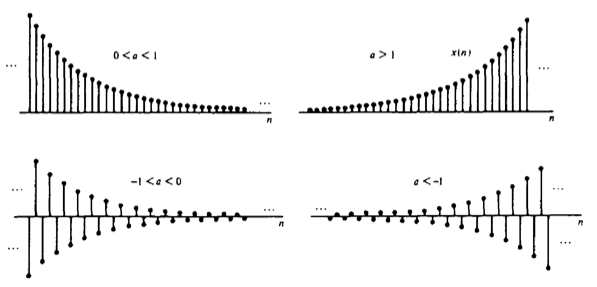
\includegraphics[width=10cm]{exp}
	\caption{Exponential Signals}
	\end{figure}
	
	\subsection{Classification of DT Signals}
	\textbf{Even and Odd Signals}
	
	A real valued signal is considered even (symmetric) if
	\begin{equation}
 	 x(-n) = x(n),
	\end{equation}
	and on the other hand, a signal is considered odd (anti-symmetric) if
	\begin{equation}
 	 x(-n) = -x(n).
	\end{equation}
	If a signal is odd then x(0) will always be zero. 
	
	Any arbitrary signal can be written as the sum of two signal components, one even and one odd. The two following formulas will show how to calculate the even and odd components of a signal.
	\begin{equation}
 	 x_e(n) = \frac{1}{2} [x(n) + x(-n)]
	\end{equation}
	\begin{equation}
 	 x_o(n) = \frac{1}{2} [x(n) - x(-n)]
	\end{equation}
	\begin{equation}
 	 x(n) = x_e(n) + x_o(n)
	\end{equation}
	
	\subsection{Simple Manipulations of DT Signals}
	\textbf{Transformation of the independent variable (time)}
	
	A signal x(n) may be shifted in time by replacing n with $n-k$ where k is an integer. If k is a positive integer the time shift results in a delay of the signal by k samples. If k is negative, the time shift results in an advance of the signal by $|k|$ samples. To advance a signal in time, the value must be stored in memory, since otherwise the signal hasn't be received. Another way that a signal can be manipulated is by flipping (folding) the signal be replacing n with -n. This flips the signal about the origin. The following figure illustrates the two operations. These operations are not communicative (flipping then shifting will not result in the same function as shifting then flipping). 
	\begin{figure}[h]
    \centering
	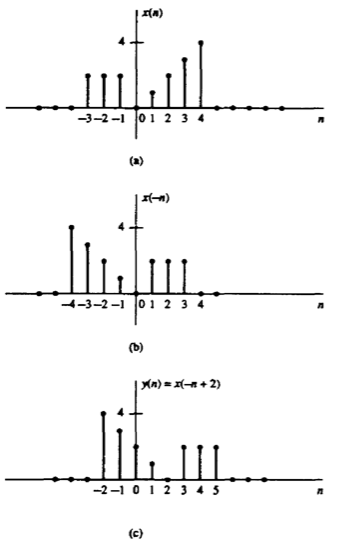
\includegraphics[width=6cm]{manip}
	\caption{Example of folding and shifting}
	\end{figure}
	
	\section{Discrete-Time Systems}
	
	Most applications of involve an algorithm that acts on the signals, which is considered the system. In general, we view a system as in operation or set of operations performed on an input signal x(n) to produce the output signal y(n). It can be said that x(n) was transformed into y(n).
	\begin{equation}
 	 y(n) = \mathcal{T}[x(n)]
	\end{equation}
	 
	\subsection{Input-Output Descriptions of Systems}
	Systems can be looked at by thinking of it as a "black box". In the following example's final form, you dont see the mathematical operations happening. That is the I-O Description. Other ways to look at a system are block diagrams.
	\textbf{Input-Output Description of Accumulator}
	\begin{equation}
 	y(n) = \sum_{k = -\infty}^n x(k) = \sum_{k = -\infty}^{n-1} x(k) + x(n)
	\end{equation}
	\begin{equation}
 	y(n) = y(n-1) + x(n)
	\end{equation}
	
	\subsection{Classification of DT Systems}
	
	In the analysis and design of systems, it is desirable to classify the systems with the proprieties they have. For a system to posses a given property, the property \textbf{MUST} hold for every possible input signal. 
	
	\textbf{Memory and Memory-less Systems}\\
	 A DT system is called memoryless (static) if its output at any $n$ depends at most on the input sample at the same time, but not on past or future samples. In any other case the system is said to have memory (or be dynamic). The following equation is memoryless, 
	\begin{equation}
 	y(n) = ax(n)
	\end{equation}
	whereas,
	\begin{equation}
 	y(n) = \sum_{k=0}^n x(n-k)
	\end{equation}
	has memory. 
	
	\textbf{Time-Invariant vs Time-Variant Systems}\\
	The general class of systems can be divided into two broad categories, time-invariant and time-variant. A system is time-invariant if its input output characteristics do not change with time. For example, a system $\mathcal{T}$ (with initial conditions = 0) has an input x(n) and produces y(n). Thus:
	\begin{equation}
 	 y(n) = \mathcal{T}[x(n)]
	\end{equation}
	Now, that same input signal is delayed by k units to yield x(n-k) and applied to the same system. If the characteristics do not change with time (time-invariant) the output will be y(n-k).\\ 
	\textbf{Definition:} A relaxed system (initial conditions = 0) $\mathcal{T}$ is time invariant if and only if 
	\begin{equation}
 	x(n) \xrightarrow[]{\mathcal{T}}  y(n)
	\end{equation}
	implies that 
	\begin{equation}
 	x(n-k) \xrightarrow[]{\mathcal{T}}  y(n-k)
	\end{equation}
	
	\textbf{Linear vs nonlinear systems} \\
	The general class of systems can also be subdivided into linear systems and non-linear systems. A linear system is one that satisfies the \textit{superposition principal}. Simply, the respose of the system to a weighted sum of singals will be equal to the corresponding weighted some of the outputs.\\
	\textbf{Definition:} A system is linear if and only if 
	\begin{equation}
 	\mathcal{T}[a_1x_1(n) + a_2x_2(n)] = a_1\mathcal{T}[x_1(n)] + a_2\mathcal{T}[x_2(n)]
	\end{equation}
	
	\textbf{Causal vs Non-Causal System Definition} \\
	A system is causal if the  output of the system at any time n depends only on the present and past inputs (x(n), x(n-1) ...) but doesnt depend on future samples (x(n+1)). 
	
	\textbf{Stable vs Unstable Systems} \\
	Stability is an important property that must be considered in any practical application of a system. Unstable systems usually behave in erratic and extreme ways that can cause overflow in a practical implementation.\\
	\textbf{Definition:} An arbitrary relaxed system is said to be bounded input - bounded output (BIBO) stable if and only if every bounded input produces a bounded output. Good example on page 67.
	\begin{equation}
 	|x(n)| \le M_x < \infty, \;\;\;\; |y(n)| \le M_y < \infty
	\end{equation}
	
	\section{Analysis of DT LTI Systems}
	Linear, time-invariant systems are characterized in the time domain by their unit sample response. The response of a LTI system to any arbitrary input can be expressed  in terms of the unit sample response of the system.
	\subsection{Techniques for the Analysis of Linear Systems}
	For a LTI system, there are generally two ways to analyze the response of the system to the input. The first method is to look the general form of the input-output relationship.
	\begin{equation}
 	y(n) = - \sum_{k=1}^N a_ky(n-k) + \sum_{k=0}^M b_k x(n-k)
	\end{equation}
	Where $a_k$ and $b_k$ are constant parameters that specify the system and are independent of x(n) and y(n). This relationship is called a \textbf{difference equation}. The other method is to decompose the input signal into a weighted sum such as
	\begin{equation}
	x(n) = \sum_k c_k x_k(n)
	\end{equation}
	where $c_k$ are the weighting coefficients of the signal x(n). Thus the response to the system y(n) from (n) is
	\begin{equation}
 	y_k(n) = \mathcal{T}[x_k(n)]
	\end{equation}
	\begin{equation}
 	y(n) = \mathcal{T}[x_k(n)] = \mathcal{T}[\sum_kc_kx_k(n)]
	\end{equation}
	\begin{equation}
 	y(n) = \sum_kc_k \mathcal{T}[x_k(n)]
	\end{equation}
	\begin{equation}
 	y(n) = \sum_kc_ky_k(n)
	\end{equation}
	
	\subsection{Resolution of DT Signal into Impulses}
	One important property when dealing with DT signals is the \textbf{sifting property}. This states that when multiplying a signal x(k) by a unit sample function at delay k will produce the sample corresponding to the delay, x(k).
	\begin{equation}
 	x(n) = \sum_{k=-\infty}^{\infty} x(k) \delta(n-k)
	\end{equation}
	
	\subsection{The Convolution Sum}
	Having resolved an arbitrary input signal x(n) into a weighted sum of impulses we can now derive the response of any \textbf{linear} system to a signal. The response of the system to a unit sample is denoted by h(n). 
	\begin{equation}
 	y(n, k) = h(n, k) = \mathcal{T}[\delta (n-k)]
	\end{equation}
	If x(n) is expressed as a sum of weighted impulses then 
	\begin{equation}
 	x(n) = \sum_{k = -\infty}^{\infty} x(k) \delta(n-k)
	\end{equation}
	Then y(n) is defined as 
	\begin{equation}
 	y(n) = \mathcal{T}[x(n)] = \mathcal{T}[\sum_{k=-\infty}^{\infty} x(k)\delta(n - k)]
	\end{equation}
	\begin{equation}
 	y(n) = \sum_{k=-\infty}^{\infty}x(k) \mathcal{T}[\delta(n - k)]
	\end{equation}
	\begin{equation}
 	y(n) = \sum_{k=-\infty}^{\infty} x(k)h(n, k)
	\end{equation}
	This shows that it follows the superposition property and is known as the \textit{superposition summation}. If the system is \textbf{time invariant} and \textbf{linear} (LTI), the impulse response simplifies considerably.
	\begin{equation}
 	h(n) = \mathcal{T}[ \delta(n)]
	\end{equation}
	By the time invariance property, the impulse response to $\delta(n-k)$ is
	\begin{equation}
 	h(n-k) = \mathcal{T}[\delta(n-k)]
	\end{equation}
	which reduces eq34 to 
	\begin{equation}
 	y(n) = \sum_{k=-\infty}^{\infty}x(k)h(n-k)
	\end{equation}
	This formula gives the response y(n) of the LTI system as a function of the input signal x(n) and the impulse response h(n). It is called the \textbf{convolution sum}. The convolution sum is calculated with the following 4 steps.
	
	\textbf{1.} Flip h(k) about k=0 to obtain h(-k)
	
	\textbf{2.} Shift h(-k) by n number of samples to obtain h(n - k)
	
	\textbf{3.} Multiply x(k) by h(n - k)
	
	\textbf{4.} Sum all the values \\
	The convolution operation is communicative in the sense that it is irrelevant which of the two sequences is folded and shifted. To summarize, convolution provides a mean for computing the response of a relaxed, LTI system to any arbitrary input signal.
	
	\subsection{Properties of Convolution and LTI Systems}

	\textbf{Commutative Law} : $x(n) \ast h(n) = h(n) \ast x(n)$ \\
	\textbf{Associative Law} : $[x(n) \ast h_1(n)] \ast h_2(n) = x(n) [h_1(n) \ast h_2(n)]$ \\
	\textbf{Distributive Law} : $ x(n) \ast [h_1(n) + h_2(n)] = x(n) \ast h_1(n) + x(n) \ast h_2(n)$ \\
	\textbf{Causal:} A LTI system is causal if and only if its impulse response is zero for negative values of n. \\
	\begin{equation}
 	y(n) = \sum_{k=0}^{\infty} h(k)x(n-k) = \sum_{k=-\infty}^n x(k)h(n-k)
	\end{equation} \\
	\textbf{Stability:} A LIT system is stable if its impulse response if absolutely summed (good examples on pg87) ie,
	\begin{equation}
 	S_h = \sum_{k=-\infty}^{\infty} |h(k)| < \infty
	\end{equation}
	
	\section{DT Systems Described by Difference Equations}
	Since Infinite Impulse Response is not able to be practically realized using convolution, the are described as \textbf{Difference Equations}. These equations take into account the current inputs and the past outputs. Most of the time this is done with a feedback loop in the system.	
	\subsection{LTI Systems Characterized by Constant-Coefficient Difference Equations}
	Systems described by constant-coefficient (CC) linear difference equations are a subclass of the recursive and nonrecursive systems introduced previously. Suppose we have a recursive system with an input-output equation
	\begin{equation}
 	y(n) = ay(n-1) + x(n)
	\end{equation}
	where a is a constant. 
	
	\begin{figure}[h]
    \centering
	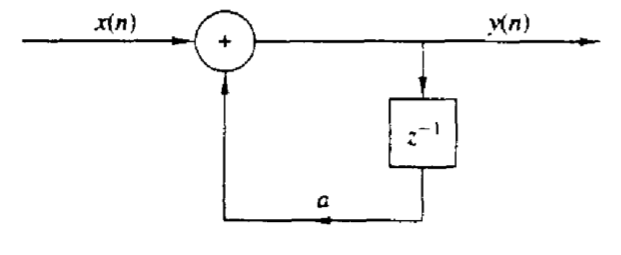
\includegraphics[width=10cm]{feed}
	\caption{Block Diagram of Recursive System}
	\end{figure}
	To solve this function it is assumed there is an initial condition for y(-1). Applying a input signal to the previous equation and solving creates:
	\begin{equation}
 	y(n) = a^{n+1}y(-1) + \sum_{k=0}^{n}a^kx(n-k)
	\end{equation}
	which is the response of the system. It consists of two parts, the term y(-1) which is a result of the initial condition and the second if the response of the system to x(n). A recursive system is relaxed if the initial conditions are zero. The zero state response is:
	\begin{equation}
 	y_{zs}(n) = \sum_{k=0}^{n}a^kx(n-k)
	\end{equation}
	and the zero input response is:
	\begin{equation}
 	y_{zi}(n) = a^{n+1}y(-1)
	\end{equation}
	The full response if 
	\begin{equation}
 	y(n) = y_{zi}(n) + y_{zs}(n)
	\end{equation}
	The previous example was a first order difference equation (simplest). The general form for a difference equation is 
	\begin{equation}
 	y(n) = -\sum_{k=1}^N a_ky(n-k) + \sum_{k=0}^{M}b_k x(n-k)
	\end{equation}
	The integer N is the order of the difference equation or system.
	
	\section{Correlation of DT Signals}
	Correlation is an operation that closely resembles convolution. Correlating two signals is a way to measure how similar the two signals are. If we have two real signals x(n) and y(n) (both have finite energy), the \textbf{cross-correlation}, $r_{xy}(l)$ is:
	\begin{equation}
 	r_{xy}(l) = \sum_{n = -\infty}^\infty x(n)y(n-l)
	\end{equation}
	or 
	\begin{equation}
 	r_{xy}(l) = \sum_{n = -\infty}^\infty x(n+l)y(n)
	\end{equation}
	The difference between convolution and correlation is that one of the signals is flipped in convolution. Hence,
	\begin{equation}
 	r_{xy}(l) = x(l) \ast y(-l)
	\end{equation}
	Since there is no flipping in correlation, it is a non-commutative operation. \textbf{Auto-correlation} is defined as,
	\begin{equation}
 	r_{xx}(l) = \sum_{n = -\infty}^\infty x(n)x(n-l)
	\end{equation}
	
\end{document} % This is the end of the document